\documentclass[11pt,pdftex,a4paper]{scrartcl}

\usepackage[utf8]{inputenc}
\usepackage{lmodern} 
\usepackage[T1]{fontenc}
\usepackage{microtype}

\usepackage[pdftex]{graphicx}
\usepackage{float}
\usepackage[hypcap]{caption}
\usepackage{subcaption}

\usepackage[pdftex]{hyperref} 
\usepackage{bookmark}

\usepackage{mathtools}
\usepackage{amssymb}
\usepackage{amsthm}
\usepackage{amsmath}

\usepackage{polski}
\usepackage[polish]{babel}
\selectlanguage{polish}

\hypersetup{
  colorlinks=true,
  urlcolor=blue,
}

\title{Stochastyczne Algorytmy Obliczeniowe}
\subtitle{ 
  Zastosowanie algorytmu genetycznego do rozwiązania problem replikacji danych
  w środowisku rozproszonym
}
\date{}
\author{
  Andrzej Kaczmarczyk
  \and
  Marcin Łoś
}

\begin{document}

\maketitle

\section{Wstęp}
Celem projektu było wybranie jednego problemu obliczeniowego, zapoznanie się z istniejącymi jego
rozwiązaniami, oraz próba ulepszenia któregoś z nich. Nasz wybór padł na problem replikacji danych
w systemach rozproszonych, oraz rozwiązanie oparte na algorytmie genetycznym, opisane w \cite{Ahmad}.

\section{Opis problemu}
Dany jest system rozproszony, składający się z \(M\) hostów \(\{H_i\}\), o pojemnościach \(s_i\), 
połączonych siecią komunikacyjną tak, że koszt przesyłu jednostki danych pomiędzy \(H_i\) i \(H_j\)
wynosi \(C(i,j)\). Istnieje także \(N\) obiektów \(\{O_i\}\), o rozmiarach \(o_i\). Host \(H_i\)
wykonuje na obiekcie \(O_k\) odpowiednio \(r^{(i)}_k\) operacji odczytu, i \(w^{(i)}_k\) operacji
zapisu. Każdy obiekt \(O_i\) znajduje się pierwotnie na jednym hoście, \(SP_i\).

Obiekty mogą zostać zreplikowane na inne hosty, tak, że suma rozmiarów obiektów zreplikowanych
na hoście \(H_i\) nie przekracza jego pojemności \(s_i\). Wszystkie hosty mają pełną wiedzę o 
replikach obiektów. Operacja odczytu obiektu \(O_k\) z hosta \(H_i\) przebiega w ten sposób, że
obiekt jest wysyłany do hosta \(H_i\) z najbliższego mu hosta zawierającego replikę \(O_k\).
Operacja zapisu natomiast odbywa się w ten sposób, że host \(H_i\) wysyła nowy stan obiektu do
hosta \(SP_k\) (pierwotnego miejsca zwierającego \(O_k\)), a ten rozsyła informację o zmianie do
pozostałych hostów zawierających repliki \(O_k\). 

Koszt sumaryczny przy danym rozłożeniu replik to suma kosztów przesyłania obiektów spowodowanego
operacjami odczytu i zapisu, przebiegającymi w opisany powyżej sposób. Koszt pojedynczego przesyłu
to iloczyn ilości przesyłanych danych (rozmiaru obiektu) i kosztu jednostkowego przesyłu między
hostami (danego przez \(C(i,j)\)). Problem polega na znalezieniu replikacji minimalizującej koszt
sumaryczny.

Nieco bardziej szczegółowy opis, wraz z wzorami na całkowity koszt znaleźć można w \cite{Ahmad}.

\section{Istniejące rozwiązania}

\section{Rozwiązanie bazowe}
Jako punkt wyjściowy przyjęliśmy rozwiązanie zaproponowane w \cite{Ahmad}.

\section{Narzędzia}
Do realizacji implementacyjnych aspektów projektu wykorzystaliśmy język Python i bibliotekę
PyEvolve \cite{pyevolve}, dostarczającą różnych komponentów (np. strategie selekcji) pozwalających
budować algorytmy genetyczne. Do implementacji rozproszonej użyte zostało MPI, za pośrednictwem
Pythonowych bindingów udostępnianych przez bibliotekę mpi4py \cite{mpi4py}.

\section{Przebieg prac}
Pierwszym celem po dokładnym zapoznaniem się z artykułem, na którym bazuje projekt, było odtworzenie
zaprezentowanych w nim wyników. W tym celu zaimplementowany został dokładnie przedstawiony w nim
algorytm (zarówno deterministyczny zachłanny -- SRA -- jak i główny -- GRA). Początkowo planowaliśmy
użyć nieco innego generatora danych do testów, takiego, który w naszym odczuciu mógłby lepiej
odwzorowywać własności instancji problemu, które występować mogą w praktyce. Dobranie jednak parametrów
tak, by zaobserwować wyniki podobne do tych przedstawionych w artykule bazowym okazało się trudne,
w związku z czym odtworzyliśmy wiernie sposób generacji danych w nim opisany. Po tym zabiegu
udało nam się odtworzyć dość dobrze oryginalne wyniki. Poniższe wykresy przedstawiają kolejno: ilość 
stworzonych replik (średnia ilość replik na obiekt), oraz zysk (jaki ułamek kosztu całkowitego
pozwoliło zaoszczędzić stworzenie replik) przy stałej ilości obiektów (150), i zmiennej ilości
hostów. Są analogiczne do tych umieszczonych w artykule bazowym, brak jednak wykresu obrazującego
zysk przy stałej ilości hostów i zmiennej ilości obiektów, ze względu na bardzo duży czas obliczeń
(wada języka Python). Algorytm genetyczny skonfigurowany był na stworzenie 10 pokoleń.

\begin{figure}[H]
    \centering
    \begin{subfigure}[b]{0.49\textwidth} 
        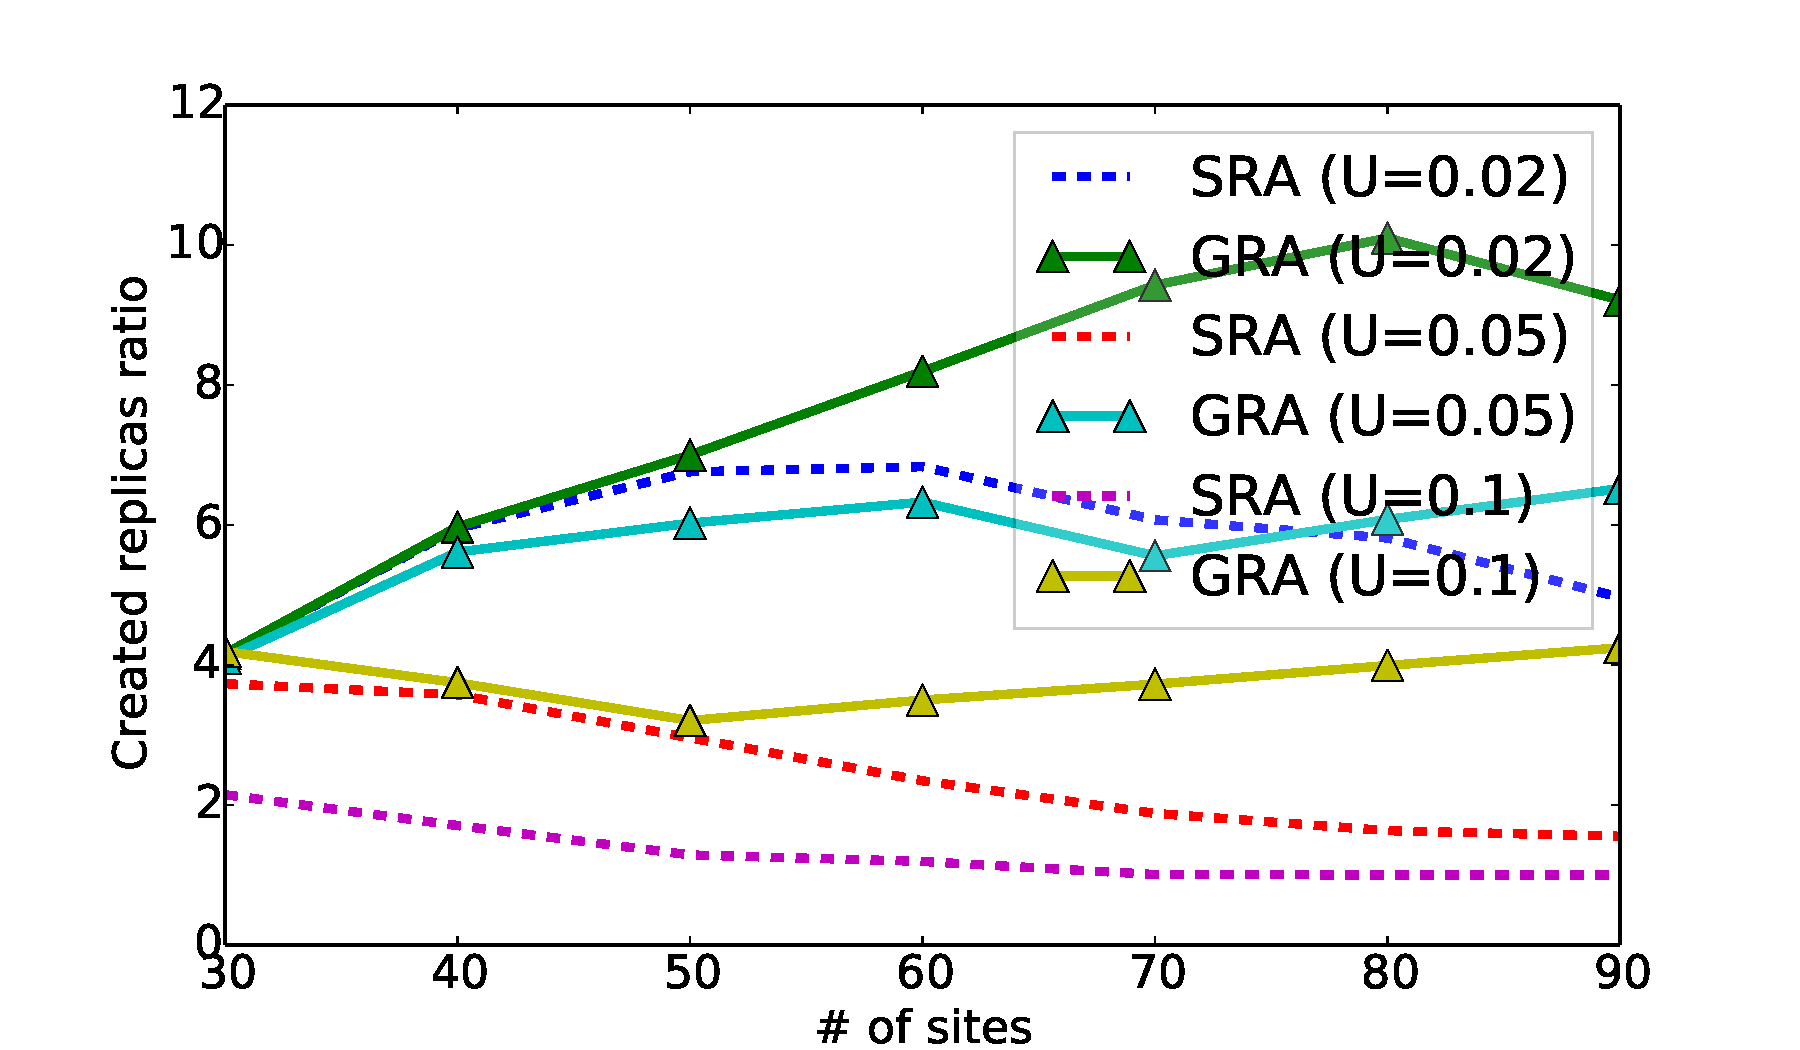
\includegraphics[width=\textwidth]{plots/replicas}
        \caption{ilość stworzonych replik}
    \end{subfigure}
    \begin{subfigure}[b]{0.49\textwidth}
        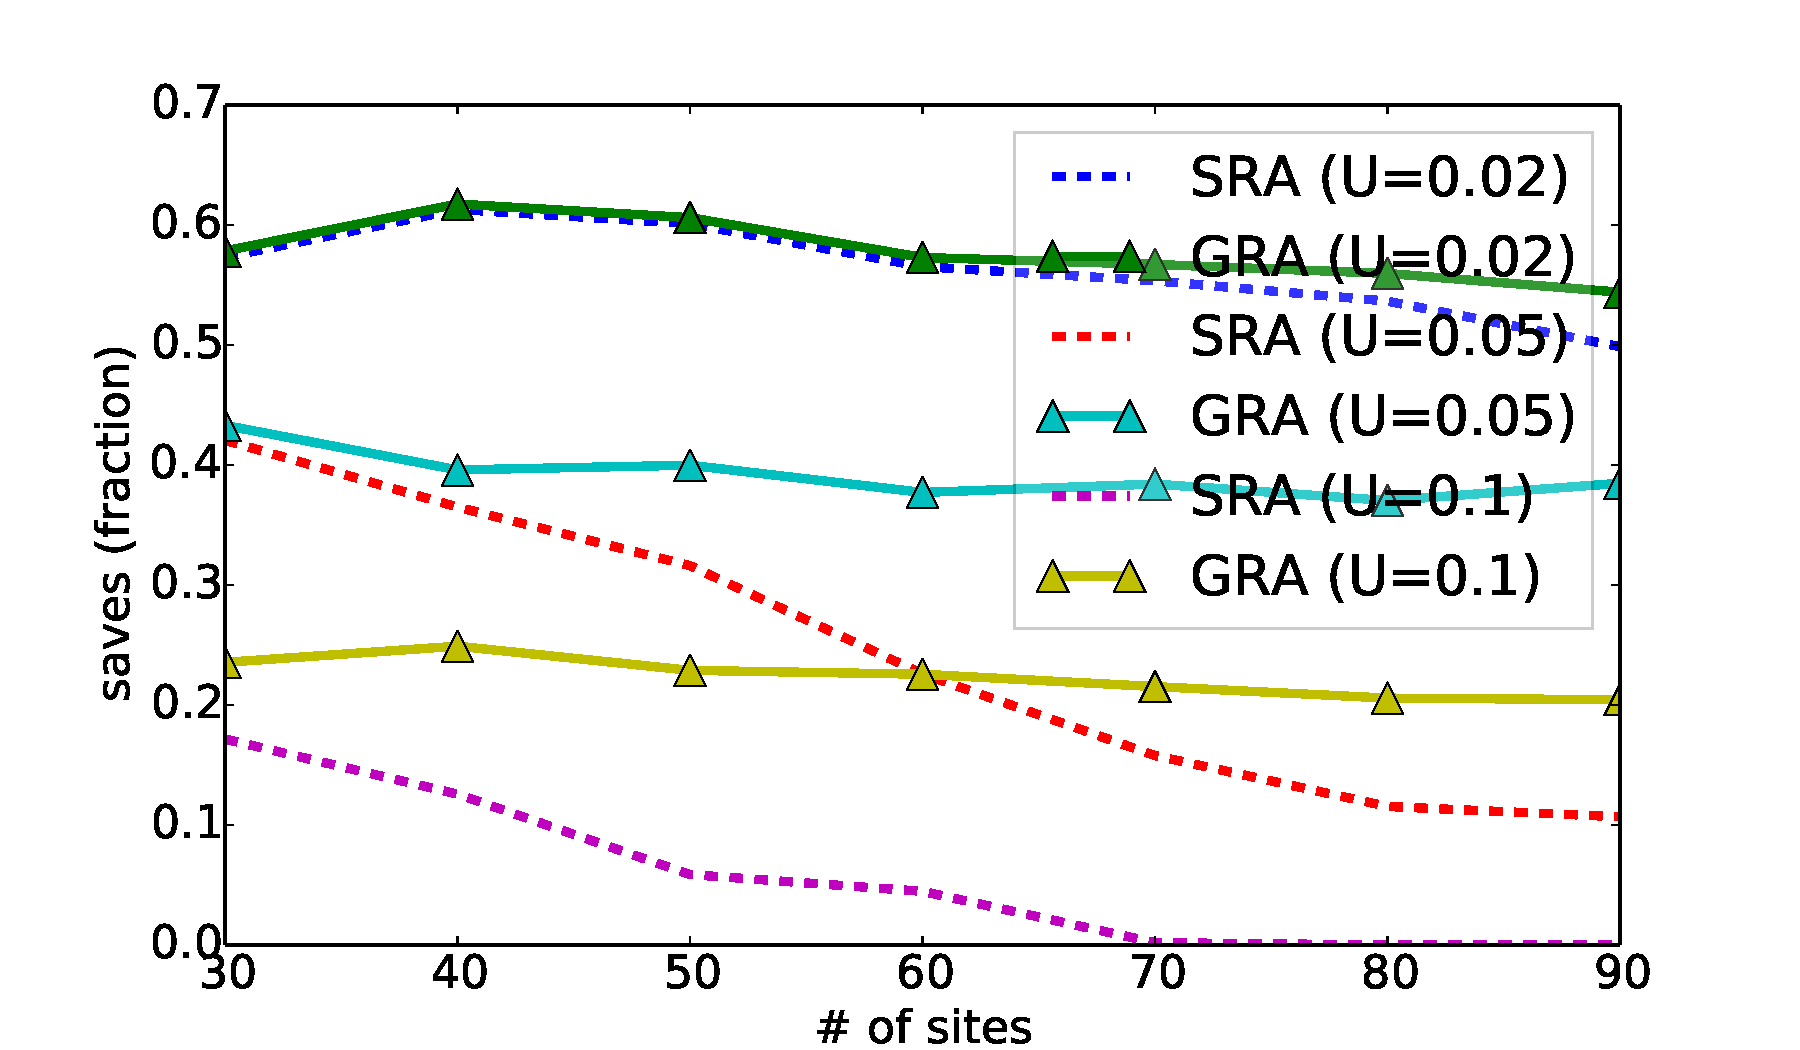
\includegraphics[width=\textwidth]{plots/saves}
        \caption{skalowane}
    \end{subfigure}

    \caption{Wyniki dla algorytmu z artykułu}
    \label{plot:original}
\end{figure}

Następnie przystąpiliśmy do stworzenia wielopopulacyjnej wersji algorytmu opartej na modelu wyspowym.
Ze względu na stosunkowo duże czasy obliczeń, by w rozsądnym czasie uzyskać wyniki dla odpowiednio
dużej liczby wysp, zdecydowaliśmy na zaimplementowanie algorytmu w wersji rozproszonej. Używany przez
nas framework PyEvolve posiada wbudowaną obsługę wielopopulacyjności i migracji osobników pomiędzy
populacjami, opartą na MPI, jednak na chwilę obecną zdaje się być dość mało dojrzała, i niezbyt dobrze
przetestowana -- doprowadzenie naszej implementacji do działania wymagało pewnej ingerencji w 
odpowiadające za to mechanizmy platformy. 

Testy wersji wielopopulacyjnej przeprowadzone zostały na komputerze Zeus, z użyciem 12 rdzeni (12 
populacji, po jednej na instancję programu), zasymulowane zostało 20 pokoleń.

\begin{figure}[H]
    \centering
    \begin{subfigure}[b]{0.49\textwidth} 
        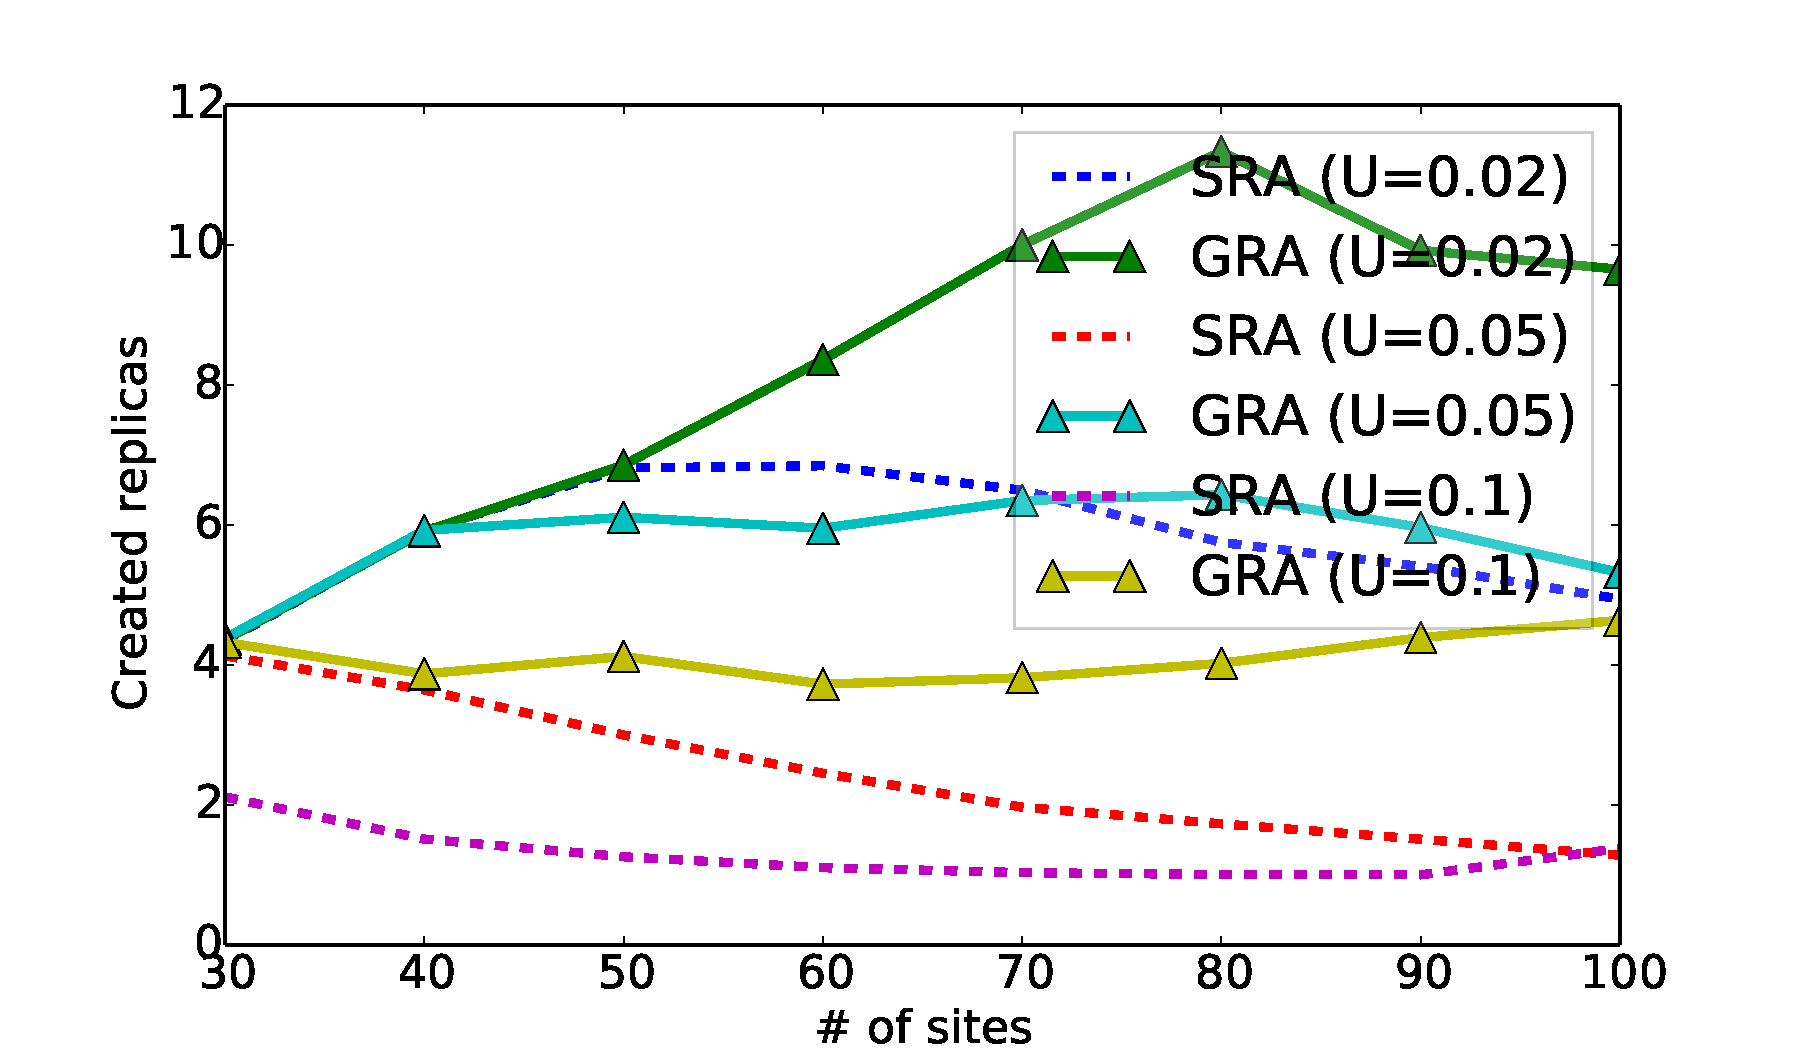
\includegraphics[width=\textwidth]{plots/replicas_isl}
        \caption{ilość stworzonych replik}
    \end{subfigure}
    \begin{subfigure}[b]{0.49\textwidth}
        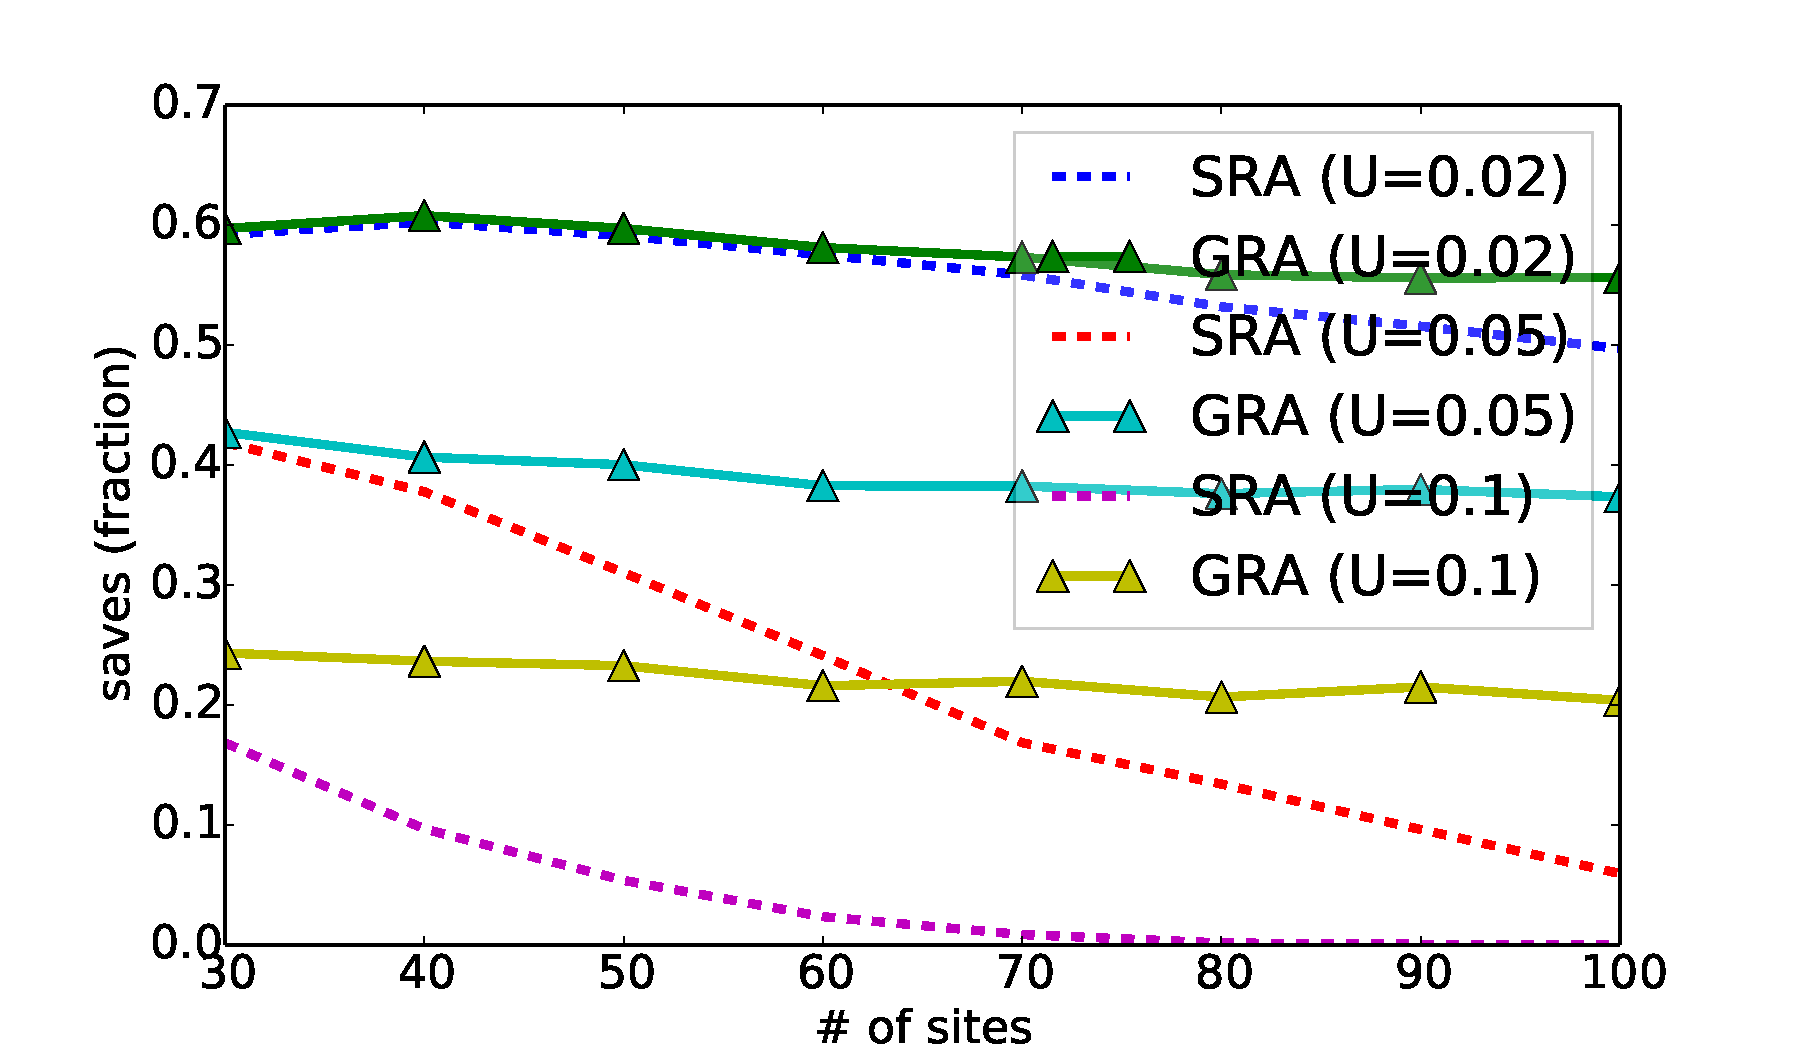
\includegraphics[width=\textwidth]{plots/saves_isl}
        \caption{skalowane}
    \end{subfigure}

    \caption{Wyniki dla algorytmu wyspowego}
    \label{plot:original}
\end{figure}

\begin{figure}[H]
    \centering
    \begin{subfigure}[b]{0.49\textwidth} 
        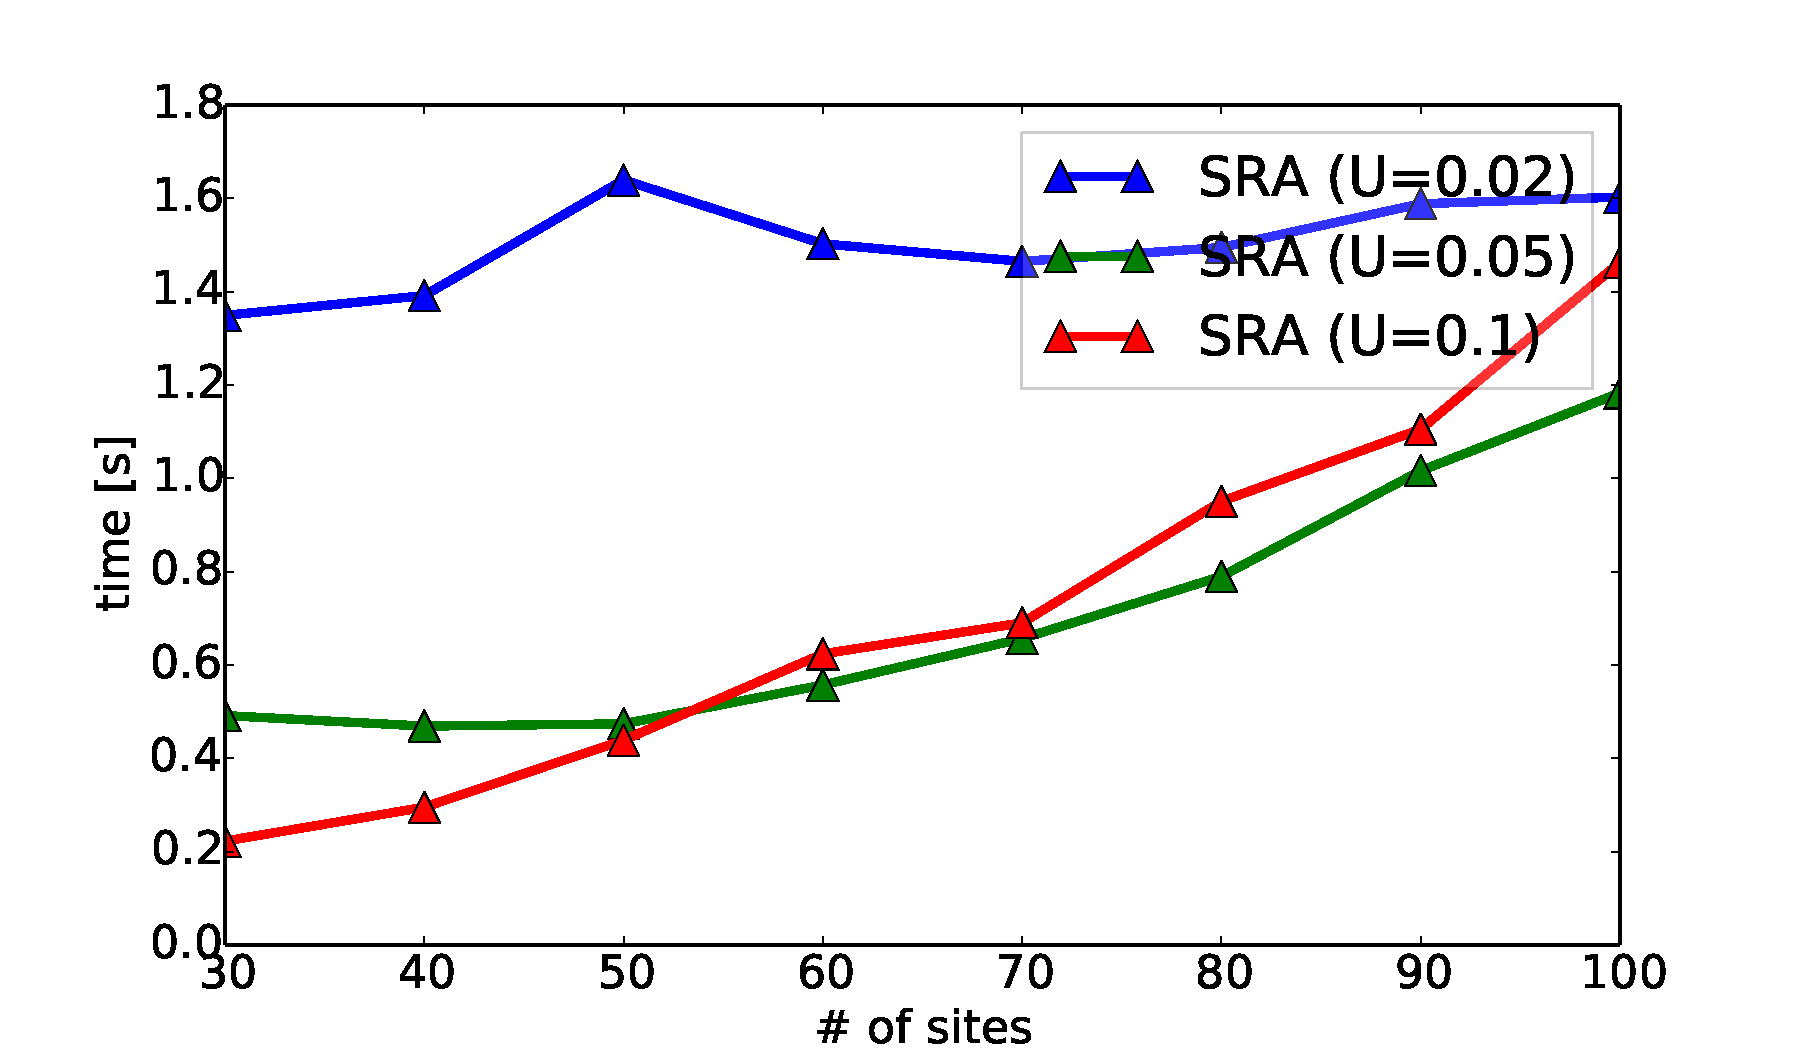
\includegraphics[width=\textwidth]{plots/time_sra_isl}
        \caption{ilość stworzonych replik}
    \end{subfigure}
    \begin{subfigure}[b]{0.49\textwidth}
        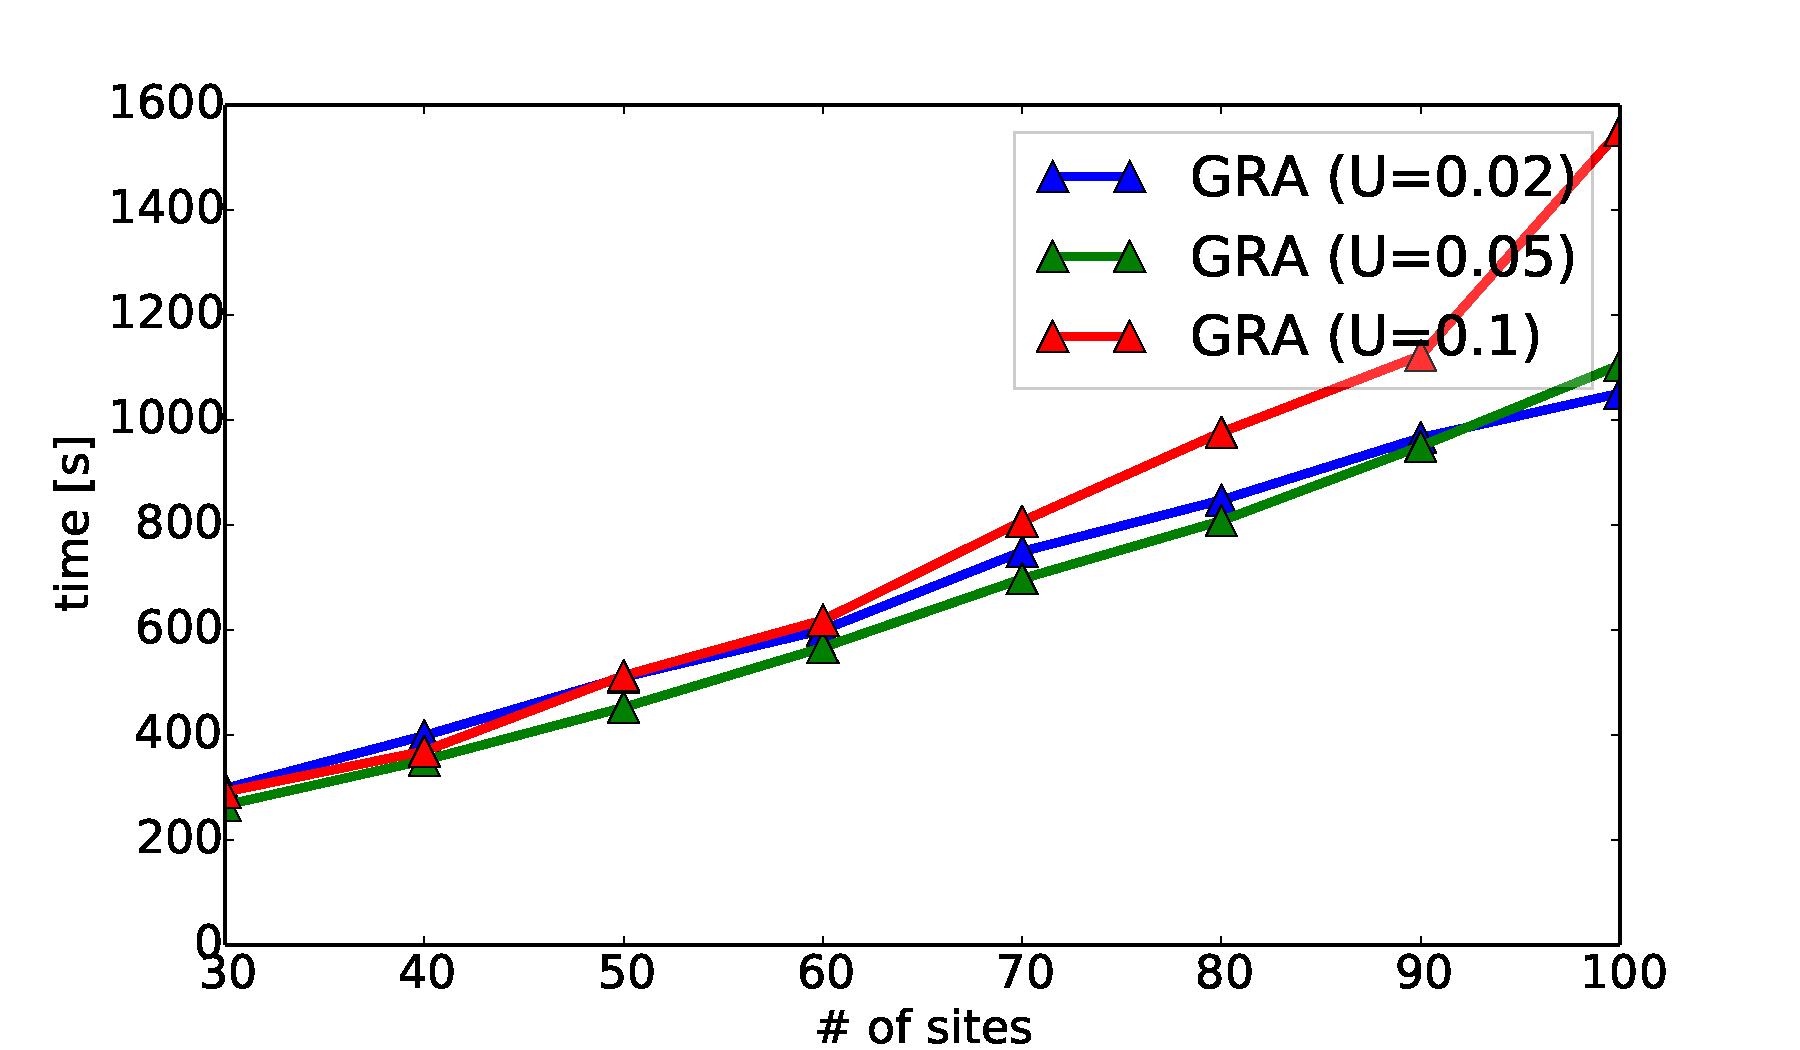
\includegraphics[width=\textwidth]{plots/time_gra_isl}
        \caption{skalowane}
    \end{subfigure}

    \caption{Czasy działania algorytmu wyspowego}
    \label{plot:original}
\end{figure}

Jak widać na powyższych wykresach, zastosowanie algorytmu wielopopulacyjnego nie przyniosło zauważalnej
poprawy w otrzymanych rozwiązaniach.

[coś o próbach redukcji do ILP]

\section{Podsumowanie}

Zastosowanie algorytmu wielopulacyjnego opartego na modelu wyspowym nie przyniosło żadnych widocznych
korzyści. Istnieje kilka możliwych przyczyn takiego stanu rzeczy. Po pierwsze, trudno powiedzieć, na
ile znajdowane rozwiązania dalekie są od rozwiązania optymalnego -- przy niewielkiej ilości operacji
zapisu algorytm obniża koszt sumaryczny o ponad połowę, niewykluczone, że rozwiązanie optymalne nie
jest znacząco od niego lepsze. Przemawia za tym także fakt, że wyniki z 10 pokoleń wersji podstawowej
i 20 pokoleń wersji wyspowej nie różnią się mimo dwukrotnego wydłużenia czasu ewolucji każdej z
populacji.

Inną możliwą przyczyną jest niewielkie zróżnicowanie populacji na poszczególnych wyspach. Populacje
wybierane są niezależnie przy użyciu tego samego schematu, i są raczej na tyle duże (80 osobników),
że trudno się spodziewać, by istotnie się od siebie różniły. Stąd, jedyną w zasadzie korzyścią z modelu
wyspowego jest zrównoleglenie obliczeń -- w pewnym sensie uruchamiamy (prawie) ten sam algorytm
na wielu maszynach, dzięki czemu mamy szansę znaleźć lepsze rozwiązanie. Nie sposób jednak oczekiwać
jakichś spektakularnych różnic.


\section{Możliwe kierunki rozwoju}

W trakcie realizacji projektu nie wszystkie pomysły zrodzone w czasie dyskusji i przemyśleń zostały
zrealizowane. Najistotniejsze kwestie są omówione w kolejnych akapitach.

Jakkolwiek algorytm wyspowy nie przyniósł żadnej obserwowalnej poprawy jakości otrzymywanych rozwiązań,
w pewnym stopniu może być to spowodowane małym zróżnicowaniem populacji na poszczególnych wyspach.
Niewykluczone, że stworzenie populacji bardziej zróżnicowanych (poprzez modyfikację rozkładów, z których
są losowane --tj. przez użycie różnych sposobów ich inicjalizowania) przyniosłoby lepszy efekt.

Jednym z pomysłów, które ostatecznie nie zostały wprowadzone w życie, była relaksacja operacji
genetycznych (mutacji i krzyżowania), polegająca na tym, by wymuszanie poprawności rozwiązań niejako
przenieść do etapu ewaluacji -- dopuszczać wszystkie stworzone osobniki, jednak stosować kary przy
ewaluacji, tak, by osobnikami o największym fitnessie były osobniki z poprawnym genotypem, jednak by
zwiększyć ,,mobilność'' populacji -- umożliwić zmiany genotypu, które bez relaksacji nie byłyby 
możliwe, i tym samym być może pozwolić na odkrycie trudnych do znalezienia minimów.

Otwarta pozostaje kwestia znalezienia lepszych operatorów mutacji i krzyżowania, bardziej dostosowanych
do rozpatrywanej przestrzeni stanów. Był to jeden z pierwszych pomysłów, jednak nie osiągnęliśmy w tym
kierunku żadnych postępów. Znalezienie sensownych operatorów wewnętrznych (nie wychodzących poza --
dość nieregularną -- przestrzeń stanów) pozwoliłoby uprościć algorytm, a ze względu na pewną 
,,kompatybilność'' z przestrzenią stanów być może także polepszyć znajdowane przez ich użycie 
rozwiązania. Wydaje się to być jednak zadanie stosunkowo trudne, i trudno na chwilę obecną powiedzieć,
jakiego rodzaju operacji można by szukać.

Przemyśleć należałoby kwestię generowania danych testowych. Nasze początkowe próby przeprowadzane
były na danych generowanych inaczej, niż w artykule, jednak wróciliśmy do niego by odtworzyć wyniki
i przy nim pozostaliśmy. Nie jest on jednak w naszym odczuciu idealny. W szczególności obiekcje 
budzić może topologię połączeń -- w artykule bazowym odległości \(C(i,j)\) pomiędzy poszczególnymi
hostami są losowane z rozkładem jednostajnym ze zbioru \(\{1,\ldots,10\}\). Najbardziej oczywistym
problemem zdaje się być pogwałcenie nierówności trójkąta -- \(C\) nie jest metryką. Trudno powiedzieć,
w jaki sposób wpływa to na używany algorytm, jednak wydaje się prawdopodobnym, że mogą istnieć jakieś
zmiany/ulepszenia, dla których jest to istotne. 

\begin{thebibliography}{}

  \bibitem{Ahmad} 
  T. Loukopoulos I. Ahmad.
  \emph{Static and Adaptive Data Replication Algorithms for Fast Information Access in 
    Large Distributed Systems}

  \bibitem{pyevolve}
  Biblioteka PyEvolve,
  \url{http://pyevolve.sourceforge.net/0_6rc1/}

  \bibitem{mpi4py}
  Biblioteka mpi4py,
  \url{http://mpi4py.scipy.org/}

\end{thebibliography}

\end{document}